\documentclass{beamer}
%\documentclass[handout]{beamer}

\mode<presentation>
{
 \usetheme{Madrid}
 \usecolortheme{beaver}
 \setbeamercovered{invisible}
}
\beamertemplatenavigationsymbolsempty
\setbeamertemplate{footline}[frame number]{}
\setbeamertemplate{blocks}[shadow=true]

% packages
\hypersetup{hidelinks}
\usepackage{placeins}
\usepackage[format=plain,
            labelfont={bf,it},
            textfont=it]{caption}
\setlength{\captionmargin}{0.3in}
\usepackage{mathtools}
\usepackage{amsthm}
\usepackage{amssymb}
\usepackage{cancel}
\usepackage[italicdiff]{physics}
% \usepackage{tocloft}
\usepackage{dsfont}
\usepackage{thmtools}
\usepackage{graphicx}
% \usepackage{longtable}

\usepackage{tikz}
\usetikzlibrary{bayesnet}

\setlength{\marginparwidth}{0.75in}

\allowdisplaybreaks

% paper-specific
\renewcommand{\vec}{\mathrm{vec}}
\newcommand{\proj}{\mathrm{proj}}

\newcommand\numberthis{\addtocounter{equation}{1}\tag{\theequation}}

\newcommand{\m}[1]{\begin{pmatrix}#1\end{pmatrix}}  % a matrix or vector
\newcommand{\sm}[1]{\begin{psmallmatrix}#1\end{psmallmatrix}}
\newcommand{\f}[1]{\frac{\StrBefore{#1}{/}}{\StrBehind{#1}{/}}} % easier fractions
\renewcommand{\sf}[1]{\tfrac{\StrBefore{#1}{/}}{\StrBehind{#1}{/}}}
\newcommand{\half}{\frac{1}{2}}
\newcommand{\thalf}{\tfrac{1}{2}}
\newcommand{\third}{\frac{1}{3}}
\newcommand{\quarter}{\frac{1}{4}}

\newcommand{\eps}{\varepsilon}
\newcommand{\clos}[1]{\overline{#1}}
\newcommand{\conj}[1]{\overline{#1}}
\newcommand{\dfeq}{\coloneqq}

\let\sp\undefined
\DeclareMathOperator{\id}{id}
\DeclareMathOperator*{\argmax}{arg\,max}
\DeclareMathOperator*{\argmin}{arg\,min}

\DeclareMathOperator{\E}{\mathbb{E}}
\let\Pr\undefined
\DeclareMathOperator{\Pr}{\mathbb{P}}
\newcommand{\indep}{\mathbin{\perp\!\!\!\!\!\:\perp}}
\newcommand{\notindep}{\mathbin{\perp\!\!\!\!\not\!\:\perp}}
\newcommand{\gvn}{\;\middle|\;}
\newcommand{\R}{\ensuremath{\mathbb{R}}}
\newcommand{\F}{\ensuremath{\mathcal{F}}}
\newcommand{\B}{\ensuremath{\mathcal{B}}}
\newcommand{\ind}{\mathds{1}}
\newcommand{\iid}{\mathrel{\stackrel{iid}{\sim}}}
\newcommand{\rv}{random variable}
\newcommand{\rvs}{random variables}
\newcommand{\iidt}{independent and identically distributed}
\newcommand{\cvp}{\xrightarrow{\:p\,}}
\newcommand{\cvw}{\xrightarrow{\,w\,}}
\newcommand{\cvd}{\xrightarrow{\,d\,}}
\newcommand{\cvas}{\xrightarrow{\;\!a.s.\:\!}}
\newcommand{\cvlp}[1]{\xrightarrow{\;\!L^{#1}\,\!}}

\DeclareMathOperator{\Var}{\mathbb{V}}
\DeclareMathOperator{\Cov}{Cov}
\DeclareMathOperator{\Corr}{Corr}
\DeclareMathOperator{\Unif}{Unif}
\DeclareMathOperator{\Expo}{Expo}
\DeclareMathOperator{\Cauchy}{Cauchy}
\DeclareMathOperator{\logit}{logit}
\newcommand{\Inv}{\mathrm{Inv-}}
\newcommand{\Pois}{\mathrm{Pois}\qty}
\newcommand{\Beta}{\mathrm{Beta}\qty}
\newcommand{\Categorical}{\mathrm{Cat}}
\newcommand{\Dirichlet}{\mathrm{Dir}\qty}
\newcommand{\Gam}{\mathrm{Gamma}\qty}
\newcommand{\Wei}{\mathrm{Wei}\qty}
\newcommand{\Hyper}{\mathrm{HGeom}\qty}
\newcommand{\Binom}{\mathrm{Bin}\qty}
\newcommand{\NBinom}{\mathrm{NBin}\qty}
\newcommand{\Multinom}{\mathrm{Multinom}\qty}
\newcommand{\Bern}{\mathrm{Bern}\qty}
\newcommand{\Bernoulli}{\mathrm{Bernoulli}\qty}
\newcommand{\Norm}{\mathcal{N}\qty}
\newcommand{\MVNorm}[1][]{\mathcal{N}_{#1}\qty}
\DeclareMathOperator{\Student}{Student-\mathit{t}}

\DeclarePairedDelimiter\br{\langle}{\rangle}
\DeclarePairedDelimiter\ceil{\lceil}{\rceil}
\DeclarePairedDelimiter\floor{\lfloor}{\rfloor}
\DeclarePairedDelimiter\round{\lceil}{\rfloor}
\DeclarePairedDelimiter\set{\{}{\}}

\DeclareMathOperator{\sgn}{sgn}
\DeclareMathOperator{\diag}{diag}
\providecommand{\norm}[1]{\lVert#1\rVert}

\newcommand{\cS}{\mathcal{S}}
\newcommand{\cR}{\mathcal{R}}
\newcommand{\cG}{\mathcal{G}}
\newcommand{\cZ}{\mathcal{Z}}
\newcommand{\cX}{\mathcal{X}}
\newcommand{\cY}{\mathcal{Y}}
\newcommand{\cW}{\mathcal{W}}
\newcommand{\cI}{\mathcal{I}}


%%%%%%%%%%%%%%%%%%%%%%%%%%%%%%%%%%%%%%%%%%%%%%%%%%%%%%%%%%%%%%%%%%%%%%

% If you wish to uncover everything in a step-wise fashion, uncomment
% the following command:
\beamerdefaultoverlayspecification{<+->}


\newcommand{\tit}{\bf Estimating Racial Disparities when\\ Race is Not Observed}

% == titles
\title[]{\tit}

\institute[Harvard]{\large Harvard University }

\date{Keynote Talk \\ Promises and Limits of Inferring Protected-Class Data\\ for Disparate
Impact Testing of AI Systems\\
  September 8, 2023 \\  \vspace{.25in} Joint work with
  Cory McCartan, Jacob Goldin, and Daniel E. Ho } 


\author[Kosuke Imai]{\large Kosuke Imai }


% == document begins
\begin{document}

%%% Title
\frame{\titlepage}

%%% Table of Contents
% \frame{\tableofcontents}

%%% Main Contents

\section{Introduction}

\begin{frame}

  \frametitle{Motivation}

  \begin{itemize}
  \item Importance of racial disparity estimation in many fields:\\
    public health, employment, voting, criminal justice, taxation,
    housing, lending, and internet technology

    \vfill
  \item But, often individual race is not available
    \begin{itemize}
    \item law may prohibit collection of information about race
      (e.g., Equal Credit Opportunity Act)
    \item agencies and companies may not wish to collect such information
    \end{itemize}
    \vfill
  \item How should we estimate racial disparities when race is not
    observed?
    \begin{itemize}
    \item standard methods use BISG (Bayesian Improved Surname
      Geocoding)
    \item but, it has been shown that they are likely to yield biased estimates
    \end{itemize}

  \item Can we improve the standard methods and eliminate their bias? 
  \end{itemize}

\end{frame}


\begin{frame}

  \frametitle{Executive Order 13985: {\small Advancing Racial Equity and Support for Underserved Communities through the Federal Government}}

  {\small\begin{itemize}
    \item \alert{Sec. 4.  Identifying Methods to Assess Equity}. \\ The
      Director of the Office of Management and Budget (OMB) shall, in
      partnership with the heads of agencies, study methods for
      assessing whether agency policies and actions create or
      exacerbate barriers to full and equal participation by all
      eligible individuals.  The study should aim to identify the best
      methods, consistent with applicable law, to assist agencies in
      assessing equity with respect to race, ethnicity, religion,
      income, geography, gender identity, sexual orientation, and
      disability.

    \vfill
  \item \alert{Sec. 5.  Conducting an Equity Assessment in Federal
      Agencies.} \\ The head of each agency, or designee, shall, in
    consultation with the Director of OMB, select certain of the
    agency's programs and policies for a review that will assess
    whether underserved communities and their members face systemic
    barriers in accessing benefits and opportunities available
    pursuant to those policies and programs.
  \end{itemize}}

\end{frame}

\begin{frame}

\frametitle{The Setup}


\begin{itemize}
\item<1-> Data
  \begin{itemize}
  \item<1-> $Y_i$: outcome of interest 
  \item<1-> $R_i$: (unobserved) race
  \item<1-> $S_i$: surname
  \item<1-> $G_i$: residence location
  \item<1-> $X_i$: other Census variables (optional)
  \item<1-> $W_i$: covariates of interest
  \end{itemize}
\item<2-> Census data
  \begin{itemize}
  \item<2-> $\Pr(G_i = g, R_i = r, X_i = x)$
  \item<2-> $\Pr(R_i = r, S_i =s)$ for frequently occurring surnames
  \end{itemize}

  \vfill
\item<3-> Regression estimands
  \begin{itemize}
  \item<3-> short regression: $\Pr(Y_i = y \mid R_i = r)$
  \item<3-> long regression: $\Pr(Y_i = y \mid R_i = r, W_i =w)$
  \end{itemize}

\item<4-> Racial disparity estimands
  \begin{itemize}
  \item<4-> $\Pr(Y_i =y \mid R_i = r) - \Pr(Y_i = y \mid R_i = r^\prime)$ for $r
    \ne r^\prime$
  \item<4-> $\Pr(Y_i = y \mid R_i = r, W_i = w) - \Pr(Y_i = y \mid R_i = r^\prime, W_i = w)$
  \end{itemize}
\vspace{-.25in}
\end{itemize}

\end{frame}

\begin{frame}

  \frametitle{Standard Estimation Methods}
 
\begin{enumerate}
\item Predict race via \alert{BISG} (or its variant)
  \begin{itemize}
  \item Assumption: $G_i \indep  S_i \mid R_i$
  \item Bayes rule:
    \begin{align*}
      \hat{P}_{ir} \ & = \ \Pr(R_i = r \mid G_i = g, S_i = s) \\
      \onslide<3->{& = \ \frac{\Pr(S_i =s\mid
       R_i = r)\Pr(G_i =g, R_i =r)}{\sum_{r^\prime} \Pr(S_i =s\mid
       R_i = r^\prime)\Pr(G_i =g, R_i =r^\prime)}}
    \end{align*}
  \item<4-> {\sc wru} software package {\scriptsize (Imai and Kahna 2016)}
  \end{itemize}
  \vfill
\item<5-> Estimate racial disparities $\mu_{Y\mid R}(y \mid r) = \Pr(Y_i = y \mid R_i = r)$
  \begin{itemize}
  \item<6-> \alert{weighting}:
    $$\hat\mu_{Y\mid R}^{\text{wtd}}(y \mid r) \ = \ \frac{\sum_i \mathbf{1}\{Y_i = y\}\hat{P}_{ir} }{\sum_i \hat{P}_{ir}}$$
  \item<7-> \alert{thresholding}: use the racial group with the largest
    probability as imputed race
  \end{itemize}
\end{enumerate}

\end{frame}

\begin{frame}

  \frametitle{BISG Prediction Works Reasonably Well {\scriptsize (Imai
      et al. 2022. {\it Sci. Adv.})}}

  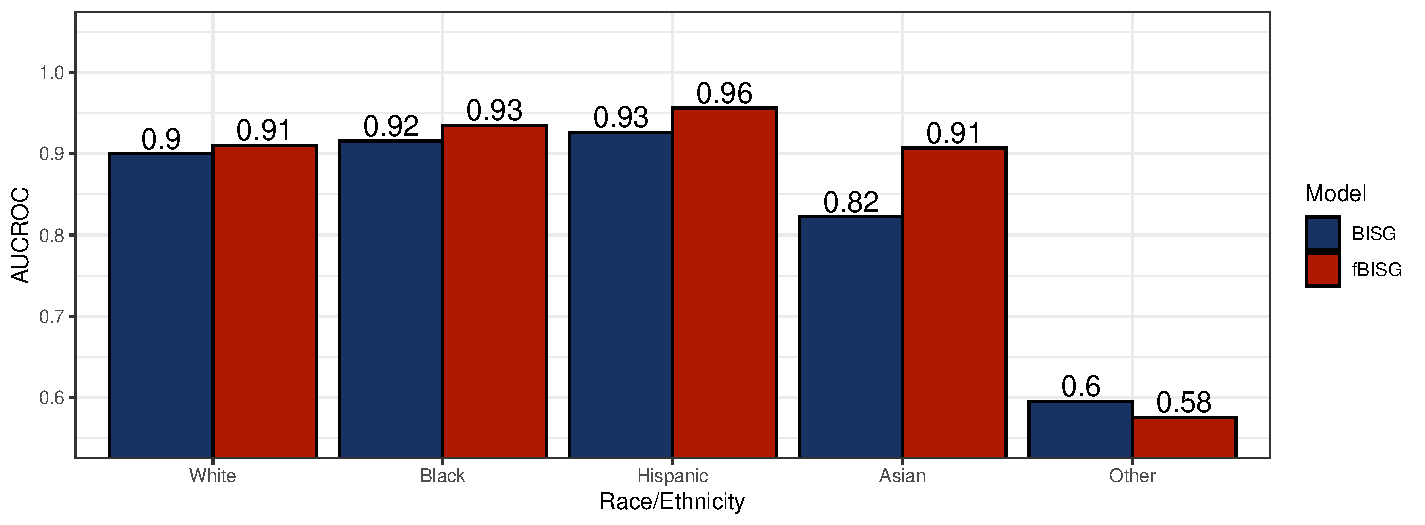
\includegraphics[width=\textwidth]{figs/AUCROC_Surnames.pdf}\\
  \onslide<2->{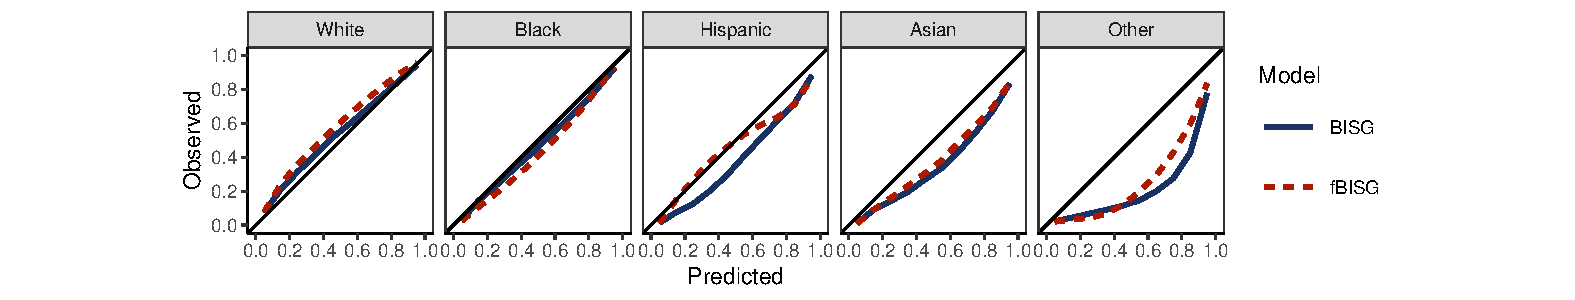
\includegraphics[width=1.2\textwidth, trim = 100 0 0 0, clip]{figs/Calibration_Surnames.pdf}}

\end{frame}

\begin{frame}

  \frametitle{Good Race Prediction Can Bias Racial
    Disparity Estimates}


  \begin{columns}
    \begin{column}{0.65\textwidth}
      \begin{itemize}
      \item<1-> Bias of the weighted estimator {\scriptsize (Chen {\it et
            al.} 2019)}
        \begin{align*}
          & \hat\mu_{Y\mid R}^{\text{wtd}}(y \mid r) - \Pr(Y_i = y
            \mid R_i = r) \\
= & - \frac{\E[\text{Cov}(\mathbf{1}\{Y_i = y\}, \mathbf{1}\{R_i = r\}\mid G_i,
          X_i, S_i)]}{\Pr(R_i = r)}
          \end{align*}
          \begin{itemize}
          \item<3-> bias tends to be large for minority groups
          \item<4-> racial disparity tends to be underestimated
          \end{itemize}
          \vfill
        \item<5-> Required assumption: $$Y_i \indep R_i \mid G_i, S_i, X_i$$
      \end{itemize}
    \end{column}
    \onslide<5->{\begin{column}{0.425\textwidth}
      \tikzstyle{main node}=[circle,draw,font=\sffamily\Large\bfseries]
      \tikzstyle{sub node}=[circle,draw,dashed,font=\sffamily\Large\bfseries]
      \hspace{-.2in}\begin{tikzpicture}[->,>=stealth',shorten >=1pt,auto,node distance=2.6cm,thick]
        
        \node[main node] (G) {$G$};
        \node[main node] (Y) [right of=G] {$Y$};
        \node[main node] (S) [below left=1.3cm and 1.3cm of Y] {$S$};
        \node[sub node] (R) [below left=0.8cm and 0.8cm of S] {$R$};
        \node[main node] (X) [below of=Y] {$X$};
        
        \path[every node/.style={font=\sffamily\small}]
        (R) edge node  {} (G)
        (R) edge node  {} (X)
        (S) edge node  {} (Y)
        (R) edge node  {} (S)
        (G) edge node  {} (X)
        (G) edge node  {} (Y)
        (X) edge node  {} (Y);
    \end{tikzpicture}
  \end{column}}
  \end{columns}
\onslide<6->{Problem: race affects many aspects of the society}

\end{frame}

\begin{frame}

  \frametitle{BIRDiE {\small (Bayesian Instrumental Regression for Disparity 
    Estimation)}}

  \begin{columns}
    \begin{column}{0.35\textwidth}
      \tikzstyle{main node}=[circle,draw,font=\sffamily\Large\bfseries]
      \tikzstyle{sub node}=[circle,draw,dashed,font=\sffamily\Large\bfseries]
   \begin{tikzpicture}[->,>=stealth',shorten >=1pt,auto,node distance=2.5cm,thick]
    
        \node[main node] (G) {$G$};
        \node[sub node] (R) [below of=G] {$R$};
        \node[main node] (S) [below left=0.5cm and 0.5cm of R] {$S$};
        \node[main node] (Y) [right of=G] {$Y$};
        \node[main node] (X) [below of=Y] {$X$};
        
        \path[every node/.style={font=\sffamily\small}]
        (R) edge node  {} (G)
        (R) edge node  {} (X)
        (R) edge node  {} (Y)
        (R) edge node  {} (S)
        (G) edge node  {} (X)
        (G) edge node  {} (Y)
        (X) edge node  {} (Y);
        
        %\path[every node/.style={font=\sffamily\small}, <->]
        %(G) edge [dashed, bend right] node  {} (S)
        %(X) edge [dashed, bend left] node  {} (S);
    \end{tikzpicture}
  \end{column}
   \begin{column}{0.65\textwidth}
      \begin{itemize}
        \item<2-> Required assumption: $$Y_i \indep S_i \mid G_i, R_i, X_i$$
        \item Race can directly or indirectly affects the outcome

          \bigskip
        \item Potential violations:
          \begin{itemize}
          \item name-based discrimination within a racial group
          \item racial categories being too coarse
         \end{itemize}
       \item The assumption holds for:
         \begin{itemize}
         \item anonymous applications
         \item algorithmic decisions without use of names
         \end{itemize}
      \end{itemize}
    \end{column}
  \end{columns}
  \bigskip
  \begin{itemize}
  \item BIRDiE incorporates BISG and its variable, estimates racial
    disparity, and produces improved race probabilities
  \end{itemize}
\end{frame}



\begin{frame}

  \frametitle{Incorporating Finer Racial Categories}

  \begin{itemize}
  \item Suppose we can have information about finer ethnic groups $f$
    \begin{itemize}
    \item $f(\text{Imai}) = \text{Japanese}$,  $f(\text{McCartan}) =
      \text{Irish}$, etc.
    \item Assume instead
      $$Y_i\indep S_i\mid \alert{f(S_i)},R_i,G_i,X_i$$
    \item Can include $f(S_i)$ as a covariate in BIRDiE
    \end{itemize}

    \vfill
  \item 1930 Census provides 22 groups
    \begin{itemize}
    \item Anglosphere and Black surname (third-or-more generation
      Whites and Blacks): Smith, Williams, Brown,
      ...
    \item First wave European immigration (German, Nordic, and Irish): Burns, Olson, Wagner, ...
    \item East Asian (Chinese, Japanese, Korean), South Asian
      (Indian, Southwest Asian),
      Southeast Asian and Pacific (Vietnamese, Filipino)
    \item Non-Cuban Hispanic (Mexican, Latin American), Cuban 
    \end{itemize}
 \end{itemize}


\end{frame}

\begin{frame}

  \frametitle{Empirical Validation}

  \begin{itemize}
  \item 2022 North Carolina voter file: 5.8M voters with
    self-reported race
  \item Subset 1M voters $\rightsquigarrow$ negligible sampling
    uncertainty

    \vfill
  \item Focus on party registration

  \end{itemize}
  \onslide<4->{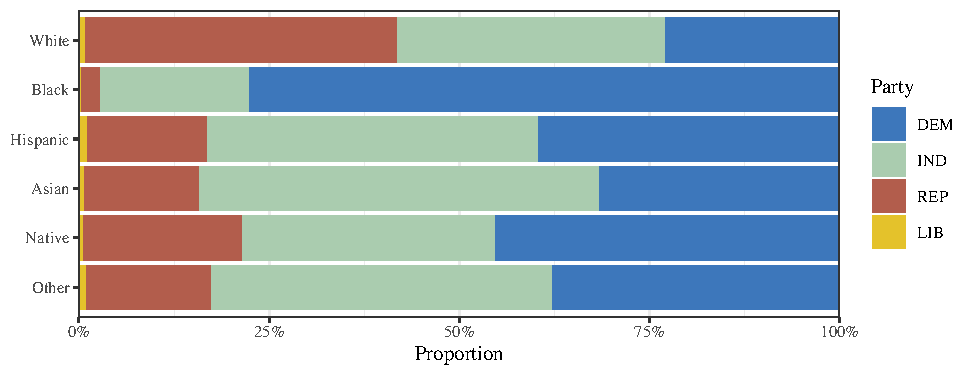
\includegraphics[width=\textwidth]{../paper/figures/nc_overview.pdf}}

\end{frame}

\begin{frame}

  \frametitle{Estimates of Racial Disparity in Party Registration}

  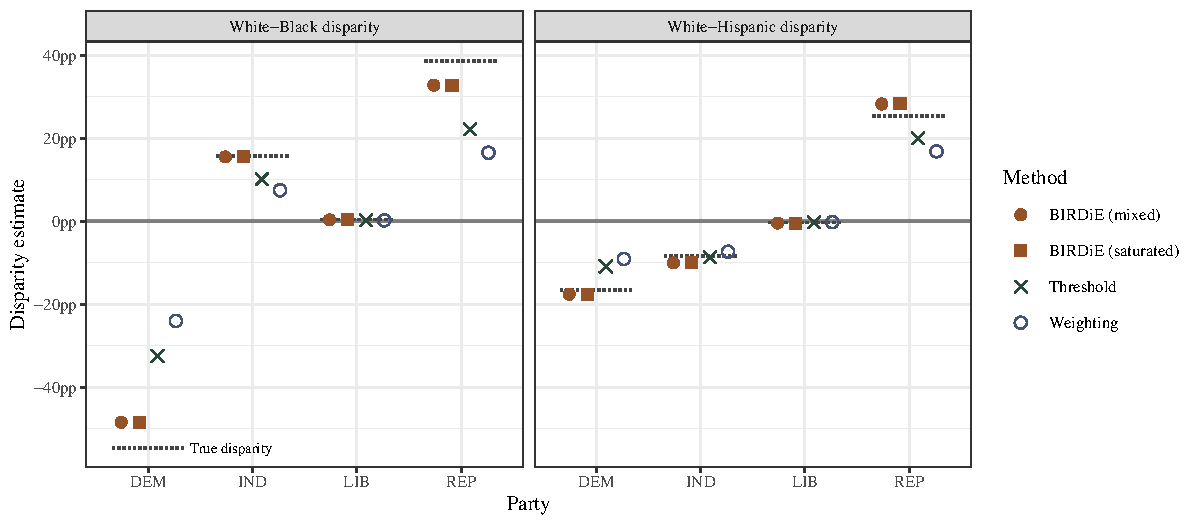
\includegraphics[width=\textwidth]{../paper/figures/nc_disp.pdf}


\end{frame}


\begin{frame}

  \frametitle{Total Variation Distance}

  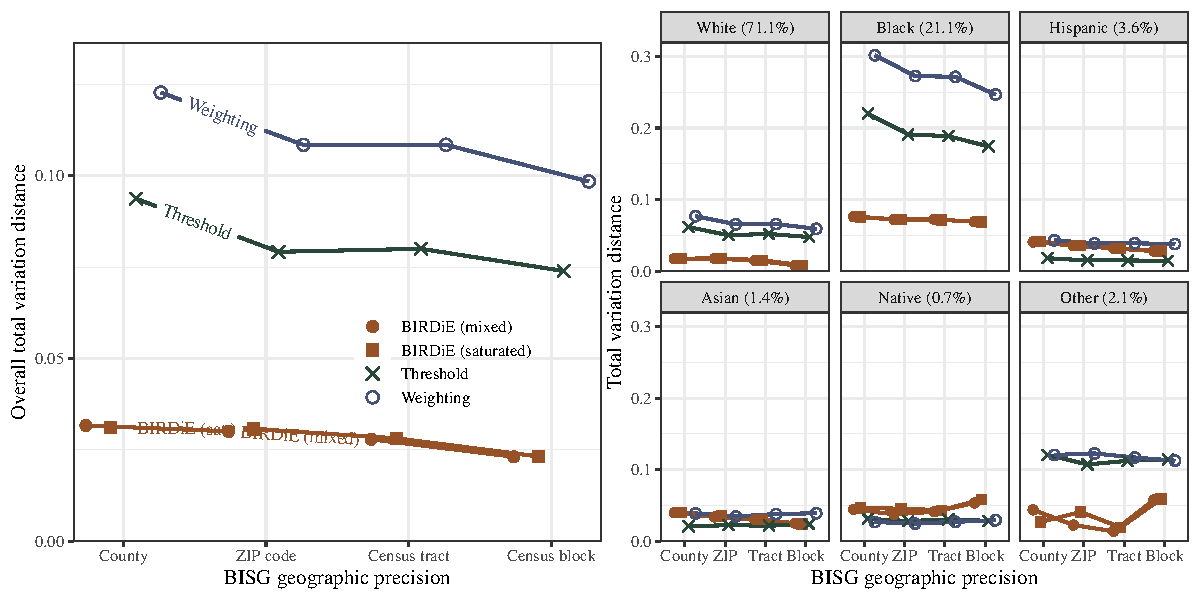
\includegraphics[width=\textwidth]{../paper/figures/nc_tv.pdf}

\end{frame}

\begin{frame}

  \frametitle{Small Area Estimation}

 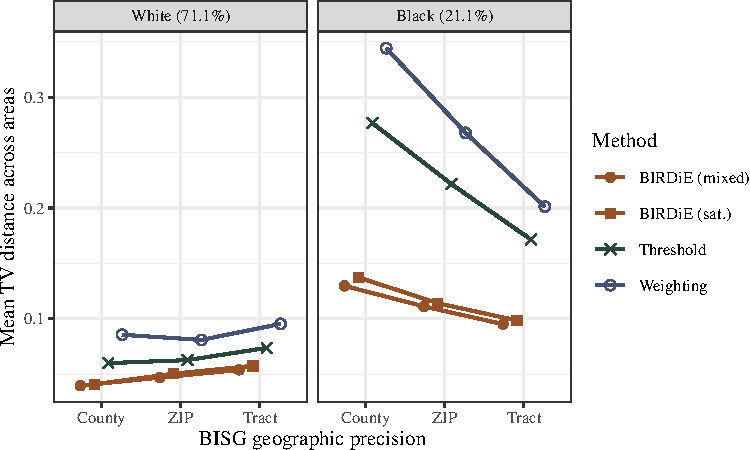
\includegraphics[width=\textwidth]{../paper/figures/nc_smallarea.pdf}


\end{frame}

\begin{frame}

  \frametitle{Improved Race Probabilities}

 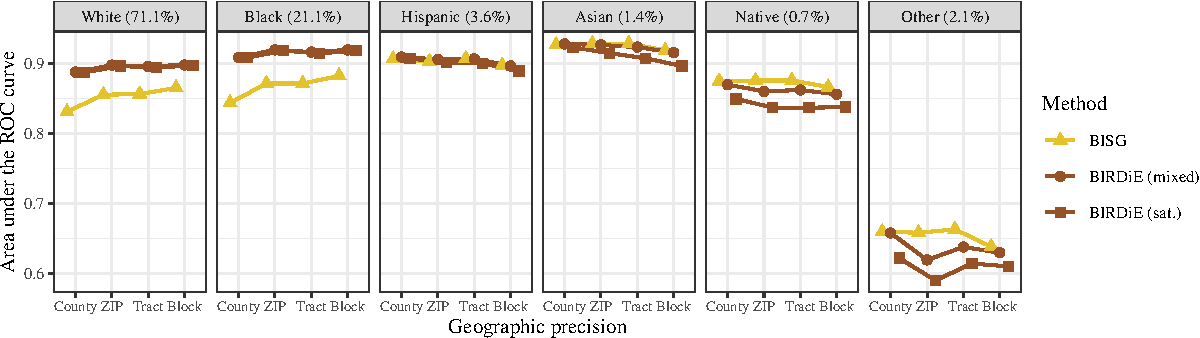
\includegraphics[width=\textwidth]{../paper/figures/nc_roc.pdf}


\end{frame}

\begin{frame}

  \frametitle{Concluding Remarks}

  \begin{itemize}
  \item BIRDiE
    \begin{itemize}
    \item new identification assumption
    \item flexible modeling with scalable estimation
    \item improved BISG race probabilities
    \item sensitivity analysis with finer racial categories
    \end{itemize}
    \vfill

  \item Future work
    \begin{itemize}
    \item collaboration with IRS: racial disparity in tax system
    \item additional empirical validations: understanding bias
    \item generalization to record linkage and data combination
    \item better use of auxiliary information in sensitivity analysis
%    \item make BIRDiE more robust to small bias in BISG probabilities
    \end{itemize}
  \end{itemize}

  \vfill
  \onslide<10->{\begin{center}
    The paper is available at
    \alert{\url{https://imai.fas.harvard.edu/research/birdie.html}} \\
    \vfill
    The software is available at \\
    \alert{\url{https://corymccartan.com/birdie/}} 
  \end{center}}
  \vspace{-.7in}
  \begin{flushright}
     
\includegraphics[scale=0.165]{../man/figures/logo.png}
  \end{flushright}
\end{frame}


\end{document}